\documentclass{kul-ulille-beamer}
%\setbeameroption{show notes on second screen=right} % Both


%% Preamble ===================================================================
\usepackage{defense}

\addbibresource{references.bib}

\title{%
  A visual Brain-Computer Interface \\
  for gaze-free communication
}
\author{Arne Van Den Kerchove}
\date{December 16, 2024}

\begin{document}

% =============================================================================

\titleframe

% =============================================================================

\begin{frame}
  \frametitle{The Locked-in Syndrome}
  \centering

  \begin{minipage}[c]{.5\textwidth}
    \includegraphics[width=\textwidth]{figures/intro/damien-obfuscated.jpg}
  \end{minipage}\hfill%
  \begin{minipage}[c]{.4\textwidth}
    \raggedright
    Paralysis with impaired speech:
    the \emph{Locked-in Syndrome}
    \bigskip

    Due to
    \begin{itemize}
      \item Stroke
      \item Traumatic brain injury
      \item Neurodegenerative diseases
      \item \ldots
    \end{itemize}
    \bigskip

  Communication requires \\ \emph{assistive technology}
  \bigskip

  What if muscle control is insufficient?
  \end{minipage}
\end{frame}


\note{%
  \begin{itemize}
    \item Some people cannot communicate
    \item Lis:  loss of nearly all voluntary control over muscles.
    \item no speech or typing
    \item require assistive technology
    \item improve QoL
    \item like eye tracker or muscle controlled switch, depending on residual
      control and impairment cannot always use this

  \end{itemize}
}
%
\begin{frame}
  \frametitle{The Brain-Computer Interface}
  \schema{figures/intro/bci.pdf}
\end{frame}


\begin{frame}[c]
  \frametitle{Research question}
  \centering

  \begin{minipage}{.8\textwidth}
  \centering
  \huge
  How can we optimize \emph{BCI}  assistive technology design  to make it more
    \emph{efficient} and  \emph{inclusive}?
  \end{minipage}

\end{frame}

\note{
  inclusive: more people can use it
}



% =============================================================================

\outline{BCI design}{figures/outline_design.pdf}
\outline{BCI design}{figures/outline.pdf}

\begin{frame}[c]
  \frametitle{Recording the brain activity}
  \schema{figures/intro/recording_modalities.pdf}
  \hfill
  \aside{%
    \emph{EEG}  measures the \\ electrical field on the
    scalp:
    \begin{itemize}
      \item[\textcolor{mygreen}{+}] Non-invasive
      \item[\textcolor{mygreen}{+}] Cheap
      \item[\textcolor{myred}{--}] Limited resolution
      \item[\textcolor{myred}{--}] Low signal-to-noise ratio
    \end{itemize}
  }
\end{frame}



\begin{frame}
  \frametitle{BCI paradigms for communication}
  \begin{minipage}[c]{.5\textwidth}
    \footnotesize
    \sffamily
\begin{tikzpicture}[
    scale=\textwidth/3cm,
  ]
  %\useasboundingbox (-1,-1.25) rectangle (1,1);
  \pgfmathsetmacro{\margin}{.1}
  \pgfmathsetmacro{\center}{.5+.5*\margin}
  \pgfmathsetmacro{\textspacing}{.15}
  %\begin{scope}[shift={(1,1.2)}]
    % Draw axes
    \draw[mydarkgray, very thick, <->] ({-(1+\margin)}, 0) -- ({1+\margin},0);
    %\draw[mydarkgray, very thick, <->] (0,{-(1+\margin)}) -- (0,{1+\margin});

    % Draw rectangles
    \draw[draw=accent1!50, fill=white, very thick] ({-\margin}, \margin) rectangle (-1,1);
    \draw[draw=accent2, fill=white, very thick] (\margin, \margin) rectangle (1,1);
    %\draw[draw=accent3!50, fill=white, very thick] (-1, {-\margin}) rectangle (1,-1);

    %% Add text
    \node[color=accent1!50, align=left,font=\bfseries, anchor=north west, inner sep=2pt] at  (-1,1){Active};
    \node[color=accent2, align=left,font=\bfseries, anchor=north east, inner sep=2pt] at  (1,1){Reactive};
    %\node[color=accent3!50, align=left,font=\bfseries, anchor=south west, inner sep=2pt] at  (-1,-1){Passive};

    %\node[color=mydarkgray, align=center,font=\bfseries, anchor=north] at
    %(0,{-(1+\margin)}) {passive\\participation};
    %\node[color=mydarkgray, align=center,font=\bfseries, anchor=south] at
    %(0,{1+\margin}) {active\\participation};
    \node[color=mydarkgray, align=center,font=\bfseries, anchor=east] at ({-(1+\margin)}, 0) {stimulus\\independent};
    \node[color=mydarkgray, align=center,font=\bfseries, anchor=west] at ({1+\margin},0) {stimulus\\dependent};

    %% Text in rectangles
    \node[align=center] at ({-\center}, {\center-\textspacing}) {movement};
    \node[align=center] at ({-\center}, {\center+\textspacing}) {speech};
    %\node[align=center] at ({-\center}, {\center-1.5*\textspacing}) {neurofeedback};

    \node[align=center] at ({\center}, {\center-1.3*\textspacing}) {tactile};
    \node[align=center] at ({\center}, {\center}) {auditory};
    \node[align=center] at ({\center}, {\center+1.3*\textspacing}) {visual};
    %\node[align=center] at ({\center-\textspacing}, {\center-\textspacing}) {mVEP};

    %% More text
    %\node[align=center] at ({\center}, {-\center+\textspacing}) {error\\potentials};
    %\node[align=center] at ({-\center}, {-\center+\textspacing}) {attention and \\ workload detection};
    %\node[align=center] at ({-\center}, {-\center-\textspacing}) {clinical neuroimaging \\ and monitoring};
    %\node[align=center] at ({+\center}, {-\center-\textspacing})  {emotion \\ detection};
    %\node[align=center] at (0, {-\center})  {$\cdots$};
  %\end{scope}
\end{tikzpicture}

  \end{minipage}\hfill%

  \aside{%
    \small
    %\emph[accent3]{Passive} BCIs not meant for communication
      \smallskip

      \emph[accent1]{Active} BCIs
      \begin{itemize}
        \footnotesize
        \item[\textcolor{mygreen}{+}] Intuitive, self-paced
        \item[\textcolor{myred}{--}] High speed requires invasive
      \end{itemize}
      \smallskip

      \emph[accent2]{Reactive} BCIs decode reactions to attended stimuli%
      \begin{itemize}
        \footnotesize
        \item[\textcolor{myred}{--}] Less intuitive
        \item[\textcolor{mygreen}{+}] Fast stimulation
        \item[\textcolor{mygreen}{+}] Suited for EEG
      \end{itemize}
      \smallskip

      \emph{Visual reactive} BCIs are a good candidate.
    }
\end{frame}
\note{%
  \begin{itemize}
    \item passive BCIs are not meant for communication
    \item categorized participation and stimulation
    \item performing a specific task
    \item brain activity from task can be decoded
  \end{itemize}
}

\begin{frame}
  \frametitle{The visual event-related potential  paradigm}
  \begin{minipage}[c]{.4\textwidth}
    \includegraphics[width=\textwidth]{figures/intro/oddball.pdf}
    \smallskip

    \begin{tikzpicture}
      \node at (current page.north east) [%
        anchor=north east,
        text width=7cm,
        fill=white, opacity=1,
        xshift=1cm,
        yshift=-.5cm,
        thin
      ]{%
        \input{figures/intro/erp.tikz.tex}
      };
    \end{tikzpicture}

  \end{minipage}\hfill%
  \begin{minipage}[c]{.5\textwidth}
    \begin{enumerate}
      \item Stimuli flash one by one
      \smallskip
      \item Flashes evoke ERPs
      \smallskip
      \item User attends a stimulus
      \smallskip
      \item ERP components are \\ modulated by attention
      \smallskip
      \item Decode target based on \\ timing and components
    \end{enumerate}
  \end{minipage}
\end{frame}


% =============================================================================

\outline{\emph{C1.} Spatiotemporal ERP decoding}{figures/outline_decode.pdf}
\begin{frame}[c]
  \frametitle{\emph{Problem:} ERP responses can be difficult to extract}
  \begin{minipage}[c]{.5\textwidth}

    Low single-trial signal-to-noise ratio
    \begin{itemize}
      \item Machine learning models must be \\ trained to decode ERPs
    \end{itemize}
    \bigskip

    Each response is a sample with \\
    \# features $=$ \# channels $\times$ \# time points
    \begin{itemize}
      \item High number of features \\ (channels $\times$ times)
      \item Short calibration time \\ results in low sample size
    \end{itemize}
    \bigskip

    \centering
    \emph{\# features $>>$ \# samples}

  \end{minipage}\hfill%
  \begin{minipage}[c]{.4\textwidth}
    \raggedleft

    \includegraphics[width=\textwidth]{figures/bttda/tensor_st.pdf}

  \end{minipage}
\end{frame}

\begin{frame}[c]
  \frametitle{Retaining space-time structure enhances performance}
  \bigskip

  \begin{minipage}[c]{.5\textwidth}
    Data are ususally flattened \\ before classification
    \begin{itemize}
      \item   ignores channel-time point structure
    \end{itemize}
  \end{minipage}\hfill%
  \begin{minipage}[c]{.4\textwidth}
    \vfill
    \raggedleft
    \includegraphics[width=.9\textwidth]{figures/bttda/tensor_flat.pdf}
  \end{minipage}
  \bigskip
  \bigskip

  \begin{minipage}[c]{.5\textwidth}
    Assumptions on \emph{data structure}
    \begin{itemize}
      \item yield strong regularization
      \item speed up training
    \end{itemize}
  \end{minipage}\hfill%
  \begin{minipage}[c]{.4\textwidth}
    \includegraphics[width=\textwidth]{figures/bttda/tensor_st.pdf}
  \end{minipage}

\end{frame}

\begin{frame}[c]
  \frametitle{Covariance matrix regularization \\
  {\tiny\cite{VanDenKerchove2022}}}
  \begin{minipage}[c]{.3\textwidth}
  \includegraphics[width=\textwidth]{figures/decode/emp_cov_label.png}
  \end{minipage}
  $=$
  \begin{minipage}[c]{.3\textwidth}
    \begin{minipage}[c]{.4\textwidth}
      \includegraphics[width=\textwidth]{figures/decode/sp_cov_2.png}
    \end{minipage}
  $\otimes$
    \begin{minipage}[c]{.4\textwidth}
      \includegraphics[width=\textwidth]{figures/decode/tmp_cov_2.png}
    \end{minipage}
  \end{minipage}\hfill
  \aside{
    Linear decoders require covariance estimation and inversion
    \bigskip

    Imprecise due to high dimensionality
    \bigskip

    Repetitive structure can be expressed as separate space and
    time covariance
    \bigskip

    Saves computation time and improves accuracy for low data
    availability



  }


\end{frame}

\begin{frame}
  \frametitle{Tensor feature extraction {\tiny\cite{VanDenKerchovesubmitted}}}

  \begin{minipage}[t]{.35\linewidth}
    Tensor discriminant analysis
    \bigskip

		\centering
		\begin{tikzpicture}[y=-1cm]
			\begin{scope}[shift={(-1,0)}]
        \TensorThree{$\ten{X}$}{\rotatebox{90}{\small channels}}{\small times}{}{2}{2}{1}
				\node at (3.2,.5, 2) {$\rightarrow$};
				\begin{scope}[shift={(3.25,0.25)}]
					\TensorThree{$\ten{G}$}{}{}{}{1}{1}{1}
				\end{scope}
				\node at (4.2,1.25, 2) {$\downarrow$};
				\begin{scope}[shift={(3,2)}]
					\TensorTwo{\textit{clf}}{}{}{1.5}{.5}
				\end{scope}
			\end{scope}
    \end{tikzpicture}
    {\tiny\cite{Phan2010}}
	\end{minipage}\hfill%
  \vrule\hfill%
  \begin{minipage}[t]{.55\textwidth}
    Block-term tensor discriminant analysis
    \bigskip

    \centering
		\begin{tikzpicture}[y=-1cm]
			\begin{scope}[shift={(-1,0)}]
				\TensorThree{$\ten{X}$}{}{}{}{2}{2}{1}
				\node at (3.2,.5, 2) {$\rightarrow$};
				\begin{scope}[shift={(3.25,0.25)}]
					\TensorThree{$\ten{G}^{(1)}$}{}{}{}{1}{1}{1}
				\end{scope}
				\node at (5.75,.5,2) {$,\cdots,$};
				\begin{scope}[shift={(6.25,0.25)}]
					\TensorThree{$\ten{G}^{(B)}$}{}{}{}{1}{1}{1}
				\end{scope}
				\node at (4.2,1.25, 2) {$\downarrow$};
				\node at (5.7,1.25, 2) {$\downarrow$};
				\node at (7.2,1.25, 2) {$\downarrow$};
				\begin{scope}[shift={(3,2)}]
					\TensorTwo{\textit{clf}}{}{}{4.5}{.5}
				\end{scope}
			\end{scope}
    \end{tikzpicture}
    \smallskip

    \begin{minipage}[t]{.5\textwidth}
      \small
      \posi\ \ More flexible
      \smallskip

      \posi\ \ Retains structure
    \end{minipage}\hfill%
    \begin{minipage}[t]{.5\textwidth}
      \small\raggedright
      \nega\ \ More parameters
      \smallskip

      Heuristic model selection
      \smallskip

      Validated with 4 open datasets
    \end{minipage}
  \end{minipage}

\end{frame}
\note{
  Another method: consider that we keep all data in its original shape and find
  separate transformations for space and for time
}


% =============================================================================

\outline{\emph{C2.} Gaze-independence}{figures/outline_gaze.pdf}


\begin{frame}
  \frametitle{\emph{Problem:} Eye motor impairment \\  prevents gazing at targets}

  \begin{minipage}[c]{.4\textwidth}
    \raggedright
    \emph{Visual skills} related to disease \\ affect BCI
    operation
    {\tiny\cite{FriedOken2020}}
  {\small
  \begin{itemize}
    \item Discomfort fixating
    \item Restricted movement
    \item Involuntary movements
  \end{itemize}
  }
  \bigskip

  Decoding relies on \emph{visual ERP} components {\tiny\cite{Treder2010}}
	\end{minipage}\hfill%
  \begin{minipage}[c]{.4\textwidth}
		\centering
		\includegraphics[width=\textwidth]{figures/intro/covert_performance_drop/brunner_2010_line.png}

    {\tiny\cite{RonAngevin2019}}


	\end{minipage}
\end{frame}

\note{
  \begin{itemize}
    \item Explain axes
    \item Accuracy is lower when not gazing directly
    \item Even below 80\% usability threshold
  \end{itemize}

}


\begin{frame}
  \frametitle{Covert visuospatial attention experiment}

  \begin{minipage}{.6\textwidth}
    \centering

    \begin{minipage}[t]{.45\textwidth}
    \input{figures/covert/interface_3.tikz.tex}
    \end{minipage}\hfill%
    \begin{minipage}[t]{.45\textwidth}
      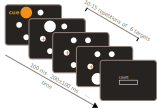
\includegraphics[width=\textwidth]{figures/covert/timeline.pdf}
    \end{minipage}
    \bigskip
    \bigskip
    \bigskip


    {\small
    \begin{minipage}{.3\textwidth}
      Overt VSA
      \smallskip

      \includegraphics[width=\textwidth]{figures/covert/attention_overt.pdf}
    \end{minipage}\hfill%
    \begin{minipage}{.3\textwidth}
      Covert VSA
      \smallskip

      \includegraphics[width=\textwidth]{figures/covert/attention_covert.pdf}
    \end{minipage}\hfill%
    \begin{minipage}{.3\textwidth}
      \small
      Split VSA
      \smallskip

      \includegraphics[width=\textwidth]{figures/covert/attention_split.pdf}
    \end{minipage}%
  }
  \end{minipage}\hfill

  \aside{%
    \small
    \raggedright
    CVSA-ERP dataset
    \begin{itemize}
      \item 15 subjects, $\pm$ 11h stimulation
      \item Hex-o-Spell interface \\ {\tiny\cite{Treder2010}}
      \item Discrete gaze-\\independence conditions
    \end{itemize}
    \raggedright
    {\tiny\cite{VanDenKerchove2024}}
  }
\end{frame}
\note{
  Hex-o-Spell optimized for gaze-independence
}

\begin{frame}
  \frametitle{Evoked ERP components}
  \small
  \begin{minipage}[t]{.45\textwidth}
    \includegraphics[width=.2\textwidth]{figures/covert/attention_overt.pdf}
    \hspace{.5em}
    \emph{Overt} VSA
    \smallskip

    \includegraphics[width=\textwidth]{figures/covert/erps/erp_overt_cluster-1.pdf}
    \includegraphics[width=\textwidth]{figures/covert/erps/erp_overt_cluster-0.pdf}
    \smallskip

    \small
    F-statistic cluster-based permutation \\ tests, target vs. non-target
  \end{minipage}\hfill%
  \begin{minipage}[t]{.45\textwidth}
    \includegraphics[width=.2\textwidth]{figures/covert/attention_covert.pdf}
    \hspace{.5em}
    \emph{Covert} VSA
    \smallskip

    \includegraphics[width=\textwidth]{figures/covert/erps/erp_covert_cluster-0.pdf}
    \smallskip

    \includegraphics[width=.2\textwidth]{figures/covert/attention_split.pdf}
    \hspace{.5em}
    \emph{Split} VSA
    \smallskip

    \includegraphics[width=\textwidth]{figures/covert/erps/erp_split_cluster-0.pdf}

  \end{minipage}
\end{frame}


%% =============================================================================

\outline{\emph{C3.} Gaze-independent decoding}{figures/outline_decode.pdf}

\begin{frame}[c]
  \frametitle{\emph{Problem:} Latency jitter decreases performance \\ in covert and split
  attention}
  \begin{minipage}{.4\textwidth}
    \centering
\small

\begin{tikzpicture}   % First subplot (low jitter) positioned relative to center
    \begin{axis}[
        at={(0,0)}, % Adjust position to the left, closer to the center
        anchor=center,
        width=\textwidth, height=.7\textwidth,
        xmin=20, xmax=80,
        ymin=-0.1, ymax=1.1,
        axis lines=none, % Remove axes
        title={low jitter}, % Add title
        title style={yshift=-10pt, color=muteblack}, % Adjust title position to make it closer to the plot
        ]
        % Plot individual waveforms (low jitter) in darkgray
        \addplot[darkgray,domain=20:80,samples=100] {exp(-0.5*((x-50)/5)^2)};
        \addplot[darkgray,domain=20:80,samples=100] {exp(-0.5*((x-52)/5)^2)};
        \addplot[darkgray,domain=20:80,samples=100] {exp(-0.5*((x-48)/5)^2)};
        \addplot[darkgray,domain=20:80,samples=100] {exp(-0.5*((x-51)/5)^2)};
        \addplot[darkgray,domain=20:80,samples=100] {exp(-0.5*((x-49)/5)^2)};

        % Plot average waveform (low jitter) in accent1 color, very thick
        \addplot[ultra thick,accent1,domain=20:80,samples=100] {exp(-0.5*((x-50)/5)^2)};
    \end{axis}
\end{tikzpicture}
\bigskip

\begin{tikzpicture}

   % Second subplot (high jitter) positioned relative to center
   \begin{axis}[
      at={(0.55\textwidth,0)}, % Adjust position to the left, closer to the center
       anchor=center,
        width=\textwidth, height=.7\textwidth,
       xmin=20, xmax=80,
       ymin=-0.1, ymax=1.1,
       axis lines=none, % Remove axes
       title={high jitter}, % Add title
       title style={yshift=-10pt, color=muteblack}, % Adjust title position to make it closer to the plot
       ]
       % Plot individual waveforms (high jitter) in darkgray
       \addplot[darkgray,domain=20:80,samples=100] {exp(-0.5*((x-45)/5)^2)};
       \addplot[darkgray,domain=20:80,samples=100] {exp(-0.5*((x-55)/5)^2)};
       \addplot[darkgray,domain=20:80,samples=100] {exp(-0.5*((x-40)/5)^2)};
       \addplot[darkgray,domain=20:80,samples=100] {exp(-0.5*((x-60)/5)^2)};
       \addplot[darkgray,domain=20:80,samples=100] {exp(-0.5*((x-50)/5)^2)};

       % Plot average waveform (high jitter) in accent1 color, very thick
       \addplot[ultra thick,accent1,domain=20:80,samples=100] {0.2*(exp(-0.5*((x-45)/5)^2) + exp(-0.5*((x-55)/5)^2) + exp(-0.5*((x-40)/5)^2) + exp(-0.5*((x-60)/5)^2) + exp(-0.5*((x-50)/5)^2))};
   \end{axis}
\end{tikzpicture}%
\bigskip

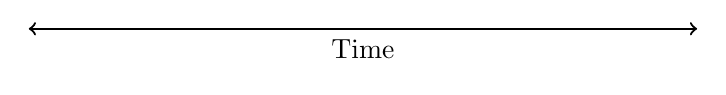
\begin{tikzpicture}
    % Draw the bottom horizontal axis
    \draw[thick,<->] (-0.35\textwidth,-1) -- (.35\textwidth,-1) node[pos=0.5,below] {Time};
\end{tikzpicture}
%\vspace{-5cm}

  \end{minipage}\hfill%
  \begin{minipage}{.55\textwidth}
    \small
    \centering
    {\centering\resizebox{.7\textwidth}{!}{%
    \small
    %CVSA-ERP (our dataset) \hspace{3.5em} BNCI2014-009
    %\smallskip

    \input{figures/covert/jitter.pgf}
    }}
    \smallskip

    \begin{itemize}
      \item Classifier-based latency estimation {\tiny\cite{Mowla2017}}
      \item Jitter of discriminative information is higher
        for gaze-independent settings
      \item Contributes to low accuracy {\tiny\cite{Arico2014}}
      \item \emph{Can this be exploited?}
    \end{itemize}

  \end{minipage}

\end{frame}
\note{
  Using a technique called CBLE extract latencies of single-trial ERPs
}

\begin{frame}
  \frametitle{Latency estimation and alignment}
  \frametitle{Latency estimation and alignment}
  \begin{minipage}{.3\textwidth}
    \emph{Before} alignment
    \smallskip

    \includegraphics[height=1.3\textwidth]{figures/covert/split_p3_latency_subject.pdf}
  \end{minipage}
  \begin{minipage}{.3\textwidth}
    \emph{After} alignment
    \smallskip

    \includegraphics[height=1.3\textwidth]{figures/covert/split_p3_latency_subject_aligned.pdf}
  \end{minipage}
  \aside{
    Developed iterative method based on CBLE
    \bigskip

    Enhances latency estimagion and SNR in simulated data
    \bigskip

    Does this transfer to real data?
  }
\end{frame}


\begin{frame}
  \frametitle{Application to gaze-independent decoding}
  \begin{minipage}{.6\textwidth}
    \centering
    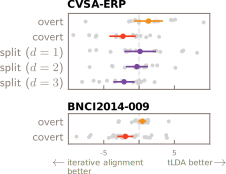
\includegraphics[width=\textwidth]{figures/covert/roc_auc_diff.pdf}
  \end{minipage}\hfill
  \aside{%
    Iterative CBLE can function with unseen data and is applicable as decoder
    \bigskip

    Within-subject, cross-validated single-trial ROC-AUC (\%)
    \bigskip

    Within and across VSA conditions to establish independence
    \bigskip

    Improves decoding performance in gaze-independent settings


  }
\end{frame}
\note{Across: transfer}

% =============================================================================

\outline{\emph{C4:} Evaluation in end-users}{figures/outline_patient.pdf}
\note{
  Now proposed a way to enhance gaze-independent decoding as a proposed
  solution for individuals with eye motor impairment
}

\begin{frame}
  \frametitle{Recruited individuals with physical, \\ speech and eye
  movement}

    \hfill
    \begin{minipage}[t]{.3\textwidth}
      3 Friedreich's \emph{ataxia}
       \begin{itemize}
          \item impaired speech
          \item involuntary eye movements
          \item discomfort fixating
        \end{itemize}
    \end{minipage}\hfill%
    \begin{minipage}[t]{.3\textwidth}
      1 bulbar onset \emph{ALS}
       \begin{itemize}
          \item no speech
          \item minor eye movement impairment
        \end{itemize}
    \end{minipage}\hfill%
    \begin{minipage}[t]{.3\textwidth}
      3 brain stem or cerebellar \emph{stroke}
       \begin{itemize}
          \item no speech
          \item partial eye paralysis
       \end{itemize}
    \end{minipage}
    \hfill
    \bigskip
    \bigskip

    \centering
    Large \emph{individual variety} in preserved skills
    \bigskip

    \hfill
    \includegraphics[height=.075\textwidth]{figures/logos/uz_leuven.jpg}
    \hfill
    \includegraphics[height=.1\textwidth]{figures/logos/chu_lille.png}
    \hfill
    \includegraphics[height=.05\textwidth]{figures/logos/trainm.png}
    \hfill
    \includegraphics[height=.1\textwidth]{figures/logos/fondation-partage-vie.png}
    \hfill
\end{frame}

\begin{frame}
  \frametitle{Off-line covert vsa experiment}

  \begin{minipage}{.6\textwidth}
    \includegraphics[height=.45\textwidth]{figures/patients/PD01a-obfuscated.jpg}%
    \hfill%
    \includegraphics[height=.45\textwidth]{figures/patients/PD01b-obfuscated.jpg}%
    \bigskip

    {\small
    \begin{minipage}{.3\textwidth}
      Overt VSA
      \smallskip

      \includegraphics[width=\textwidth]{figures/covert/attention_overt.pdf}
    \end{minipage}\hfill%
    \begin{minipage}{.3\textwidth}
      Covert VSA
      \smallskip

      \includegraphics[width=\textwidth]{figures/covert/attention_covert.pdf}
    \end{minipage}\hfill%
    \begin{minipage}{.3\textwidth}
      \small
      Free VSA
      \smallskip

      \includegraphics[width=\textwidth]{figures/covert/attention_free.pdf}
    \end{minipage}%
  }
  \end{minipage}


  \aside{
    EEG, EOG and eye-tracking
    \bigskip

    Adapted stimulation parameters
    \bigskip

    Few studies investigating VSA abilities of end-users
    \bigskip

    Replace \textit{split} by \textit{free} to study comfort

  }

\end{frame}

\begin{frame}[c]
  \frametitle{Eye tracking}
  \begin{minipage}{.6\textwidth}
    \centering
    \includegraphics[width=.8\textwidth]{figures/patients/fig_gaze.pdf}
  \end{minipage}
  \aside{
    Most prefered to perform overt VSA
    \bigskip

    Voluntary covert and split VSA did occur
    \bigskip

    Portable eye tracker not always suited

  }
\end{frame}

\begin{frame}
  \frametitle{Subject decoding performance}
  \begin{minipage}{.6\textwidth}
    \resizebox{\textwidth}{!}{
      \input{figures/patients/fig_decode.pgf}
    }
  \end{minipage}
  \aside{
    \small
    Off-line decoder comparison
    \bigskip

    All but one subject above chance
    \bigskip

    Covert was lower than overt, free generally on par
    \bigskip

    Limited impact of gaze-independent decoding
    \bigskip

    Contribution of gaze, break with limits of overt and covert

  }
\end{frame}

\begin{frame}
  \frametitle{Recap}
  \begin{enumerate}
    \item Visual, spatial ERP paradigm
    \bigskip
    \item 2 decoders exploiting spatiotemporal structure
    \bigskip
    \item Covert attention study with healthy subjects
    \bigskip
    \item Iterative alignment decoder for gaze independence
    \bigskip
    \item Off-line study with eye-motor impaired patients
  \end{enumerate}
  \aside{
    Publications
  }
\end{frame}

\begin{frame}
    \frametitle{Conclusions}
    \begin{changemargin}
    \begin{itemize}
      \item Improved decoders enhance BCI \emph{efficiency}.
      \bigskip
      \item Applications to gaze-independent decoding improve \emph{inclusivity}.
      \bigskip
      \item Limited effect on end-users
      \bigskip
      \item Gained insight in requirements of BCI users with gaze-impairment
    \end{itemize}
  \end{changemargin}
\end{frame}

\begin{frame}
  \frametitle{Perspectives}
  \begin{changemargin}
    \begin{itemize}
     \item Models capturing multi-component and
       non-stationary aspect of (covert) ERPs
     \bigskip
     \item On-line experiments
     \bigskip
     \item User experience study
     \bigskip
     \item Integrate EEG and eye-tracking
     \bigskip
  \end{itemize}
  \end{changemargin}
\end{frame}
\note{
  Once the on-line system is available, this allows us to do a proper user
  experience study
}

\begin{frame}
  \frametitle{Q\&A}

  \centering
\end{frame}
%
%%% BACKUP Slides ==============================================================



\begin{frame}[noframenumbering]
  \frametitle{Experimental procedure \\ CVSA-ERP}
  hardware, locations, timings, nr of blocks, ...
\end{frame}
\begin{frame}
  \frametitle{Experimental procedure \\ end-user study}
  hardware, locations, timings, nr of blocks, ...
\end{frame}

\begin{frame}[noframenumbering]

  \frametitle{Block-term tensor discriminant analysis procedure}
  backward model image and equation

  forward model image and equation

  deflation image and equations

  model selection procedure
\end{frame}

\begin{frame}[noframenumbering]

  \frametitle{Block-term tensor discriminant analysis procedure}
  backward model image and equation

  forward model image and equation

  deflation image and equations

  model selection procedure
\end{frame}

\begin{frame}
  \frametitle{Subjects with physical, speech and gaze impairment}

  \begin{tabular}{@{}l|lrlrl@{}}
      \textbf{ID}  & \textbf{Diagnosis} & \textbf{Age} &
      \textbf{Speech} & \textbf{Trach.} & \textbf{Communication} \\ \hline
      PA1 & bulbar-onset ALS & 58  & absent  & no          & tablet                 \\
      PB1 & Friedreich's ataxia & 41  & impaired & no          & verbal                 \\
      PB2 & Friedreich's ataxia & 43  & impaired & no          & verbal                 \\
      PB4 & Friedreich's ataxia & 48  & impaired & no          & verbal                 \\
      PC2 & brainstem stroke & 43  & absent  & yes         &  eye movement \\
      PC3 & brainstem stroke & 43  & absent  & yes         & letterboard            \\
      PC4 & cerebellar stroke & 54  & absent  & yes         & letterboard \\
  \end{tabular}

\end{frame}



\begin{frame}
  \frametitle{Eye motor impairment}
  \newcommand{\skill}{}
  \newcommand{\noskill}{x}
  \newcommand{\snoskill}{o}

  \begin{tabular}{l|ccccccc}
                            & PA1      & PB1      & PB2       & PB4      & PC2       & PC3       & PC4 \\ \hline
    \small Visual fixation         & \noskill & \noskill & \noskill  & \noskill & \noskill  & \noskill  & \noskill \\
    \small Eyelid function         & \skill   & \skill   & \skill    & \skill   &  \skill  & \noskill  & \noskill \\
    \small Ocular motility         & \skill   & \noskill & \skill    & \noskill & \snoskill & \snoskill & \noskill\\
    \small Binocular vision        & \skill   & \skill   & \skill    & \skill   & \noskill  & \snoskill & \snoskill \\
    \small Field of vision         & \skill   & \skill   & \skill    & \skill   & \skill    & \noskill  & \noskill \\
    \small Involuntary movement    & \skill   & \noskill & \snoskill  & \noskill &  \noskill  & \noskill  & \skill \\
  \end{tabular}
  \bigskip

  x: impaired, o: severely impaired
\end{frame}


\begin{frame}[c, noframenumbering]
\frametitle{User-Centered Design}

  \begin{minipage}[c]{.5\textwidth}
  \begin{tabular}{|l|l|}
    \hline
     & \emph{Principles} \\ \hline
     \emph{P1} & understand user, task, environment \\
     \emph{P2} & early and active user involvement \\
     \emph{P3} & driven by user-centered evaluation \\
     \emph{P4} & iterative design \\
     \emph{P5} & adress holistic experience \\
     \emph{P6} & multidisciplinary design \\
    \hline
  \end{tabular}
  \end{minipage}\hfill%
  \begin{minipage}[c]{.4\textwidth}
  \end{minipage}

\end{frame}


\end{document}
